% --------------------------------------------------
% --------------------------------------------------
\chapter{Tagger - Edison}
This variant of the tagger uses an Intel Edison development platform as its main computing component, in combination with two printed circuit boards with one TI MSP430G2553 microcontroller each. The Edison's main function therein is to run the control program that connects to the MSPs via $\text{I}^2\text{C}$, to the server via its onboard WiFi stack, and to the vest via an additional Grove Serial Bluetooth module.\\
Furthermore, the necessary peripherals include a \US{2.2}{\inch} TFT display, three IR reciever sensors, an IR diode, and two LED color stripes, all mounted in the tagger casing. To power all components, the tagger also includes a \SI{8}{\volt} battery pack in its grip.\\
\figref{fig:tag_ed_structure} shows the internal structure and connection of the components.

\begin{figure}[h!]
\centering
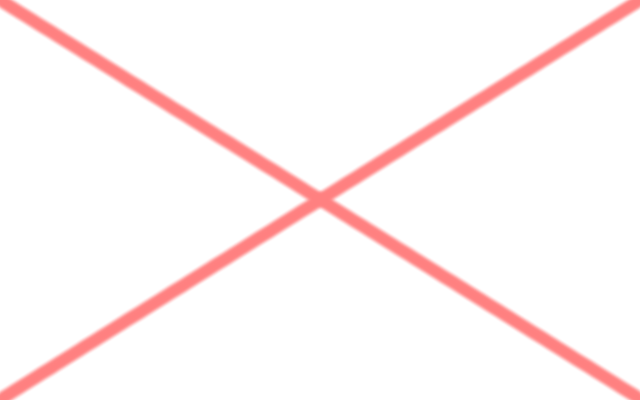
\includegraphics[width=0.75\textwidth]{images/placeholder.png}\\
\caption[Edison Tagger Structure]{Internal structure of the tagger with Edison, send/recieve PCBs, other elements and wiring.}
\label{fig:tag_ed_structure}
\end{figure}

The tagger casing consists of two grip halves and two corpus halves screwed together, with mountings for all boards, the IR recievers, and the LED stripes inside the corpus. A barrel is fixed inside the corpus and holds the IR diode and a focusing lens at its muzzle. A trigger mechanism is integrated in the grip with an electrical push-button behind it. Grip, corpus, switch and barrel are 3D printed.\\
\figref{fig:tag_ed_pic} pictures the tagger that was put together, the different components are highlighted.

\begin{figure}[h!]
\centering
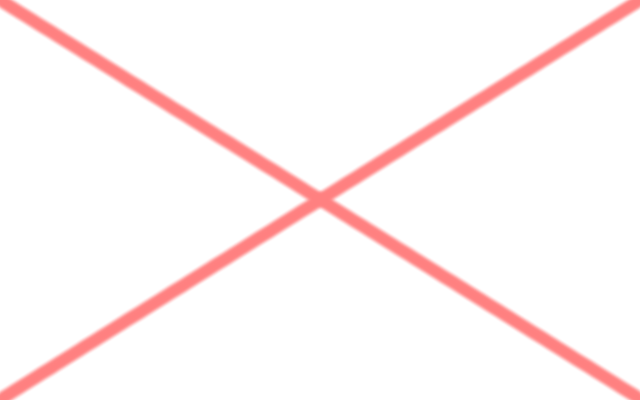
\includegraphics[width=0.75\textwidth]{images/placeholder.png}\\
\caption[Edison Tagger]{TODO: pic of tagger.}
\label{fig:tag_ed_pic}
\end{figure}

\section{Intel Edison}
\subsection{Hardware}
\subsection{Software}

\section{Send PCB}

\section{Recieve PCB}
